%%%%%%%%%%%%%%%%%%%%%%%%%%%%%%%%%%%%%%%%%
% University/School Laboratory Report
% LaTeX Template
% Version 3.1 (25/3/14)
%
% This template has been downloaded from:
% http://www.LaTeXTemplates.com
%
% Original author:
% Linux and Unix Users Group at Virginia Tech Wiki 
% (https://vtluug.org/wiki/Example_LaTeX_chem_lab_report)
%
% License:
% CC BY-NC-SA 3.0 (http://creativecommons.org/licenses/by-nc-sa/3.0/)
%
%%%%%%%%%%%%%%%%%%%%%%%%%%%%%%%%%%%%%%%%%

%----------------------------------------------------------------------------------------
%	PACKAGES AND DOCUMENT CONFIGURATIONS
%----------------------------------------------------------------------------------------

\documentclass{article}

\usepackage[utf8]{inputenc}

% Default fixed font does not support bold face
\DeclareFixedFont{\ttb}{T1}{txtt}{bx}{n}{12} % for bold
\DeclareFixedFont{\ttm}{T1}{txtt}{m}{n}{12}  % for normal

% Custom colors
\usepackage{color}
\definecolor{deepblue}{rgb}{0,0,0.5}
\definecolor{deepred}{rgb}{0.6,0,0}
\definecolor{deepgreen}{rgb}{0,0.5,0}

\usepackage{listings}

% Python style for highlighting
\newcommand\pythonstyle{\lstset{
	language=Python,
	basicstyle=\ttm,
	otherkeywords={self},             % Add keywords here
	keywordstyle=\ttb\color{deepblue},
	emph={MyClass,__init__},          % Custom highlighting
	emphstyle=\ttb\color{deepred},    % Custom highlighting style
	stringstyle=\color{deepgreen},
	frame=tb,                         % Any extra options here
	showstringspaces=false            % 
}}


% Python environment
\lstnewenvironment{python}[1][]
{
	\pythonstyle
	\lstset{#1}
}
{}

% Python for external files
\newcommand\pythonexternal[2][]{{
		\pythonstyle
		\lstinputlisting[#1]{#2}}}

% Python for inline
\newcommand\pythoninline[1]{{\pythonstyle\lstinline!#1!}}
\usepackage[version=3]{mhchem} % Package for chemical equation typesetting
\usepackage{siunitx} % Provides the \SI{}{} and \si{} command for typesetting SI units
\usepackage{graphicx} % Required for the inclusion of images
\usepackage{natbib} % Required to change bibliography style to APA
\usepackage{amsmath} % Required for some math elements 
\usepackage{diagbox}
\setlength\parindent{0pt} % Removes all indentation from paragraphs

\renewcommand{\labelenumi}{\alph{enumi}.} % Make numbering in the enumerate environment by letter rather than number (e.g. section 6)

%\usepackage{times} % Uncomment to use the Times New Roman font

%----------------------------------------------------------------------------------------
%	DOCUMENT INFORMATION
%----------------------------------------------------------------------------------------

\title{ANLP Assignment 2} % Title

\author{
	Ida \textsc{Szubert}\\
	\texttt{s0907677}
	\and
	Yue \textsc{Yu}\\
	\texttt{s1563228}
}

\date{\today} % Date for the report

\begin{document}

%----------------------------------------------------------------------------------------
%	QUESTION 2
%----------------------------------------------------------------------------------------
\section{Parse trees}
\begin{figure}[h!]
	\centering
	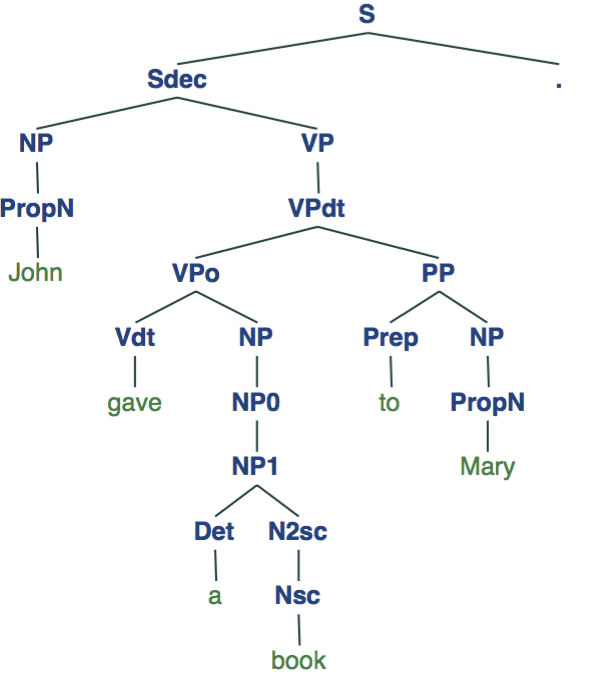
\includegraphics[width=0.4\linewidth]{../s1}
	\caption{\emph{John gave a book to Mary.}}
	\label{fig:s1}
\end{figure}
\begin{figure}[h!]
	\centering
	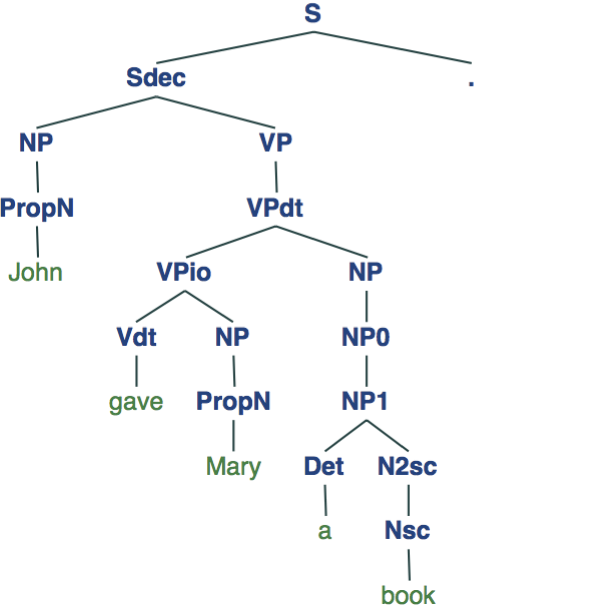
\includegraphics[width=0.4\linewidth]{../s2}
	\caption{\emph{John gave Mary a book.}}
	\label{fig:s2}
\end{figure}
\begin{figure}[h!]
	\centering
	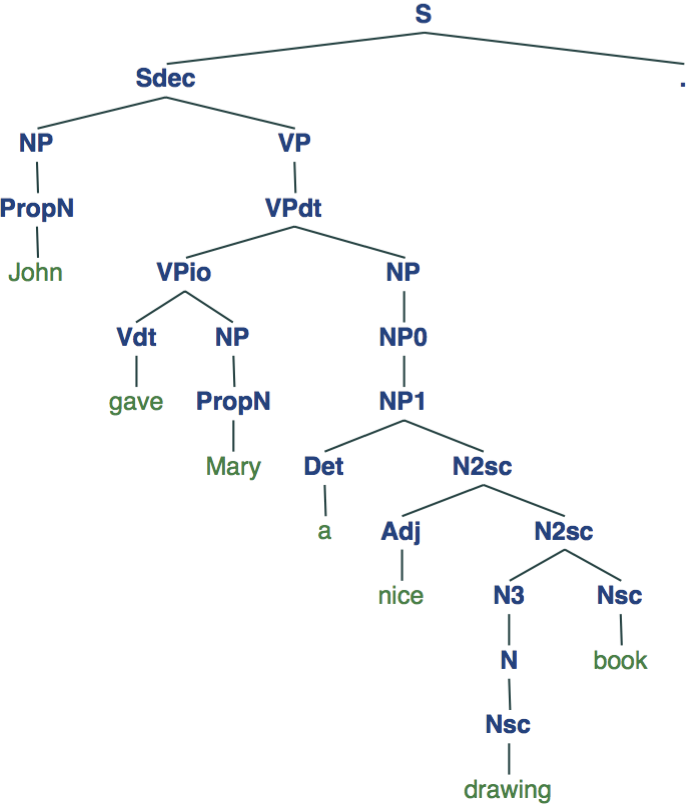
\includegraphics[width=0.4\linewidth]{../s3}
	\caption{\emph{John gave Mary a nice drawing book.}}
	\label{fig:s3}
\end{figure}
\begin{figure}[h!]
	\centering
	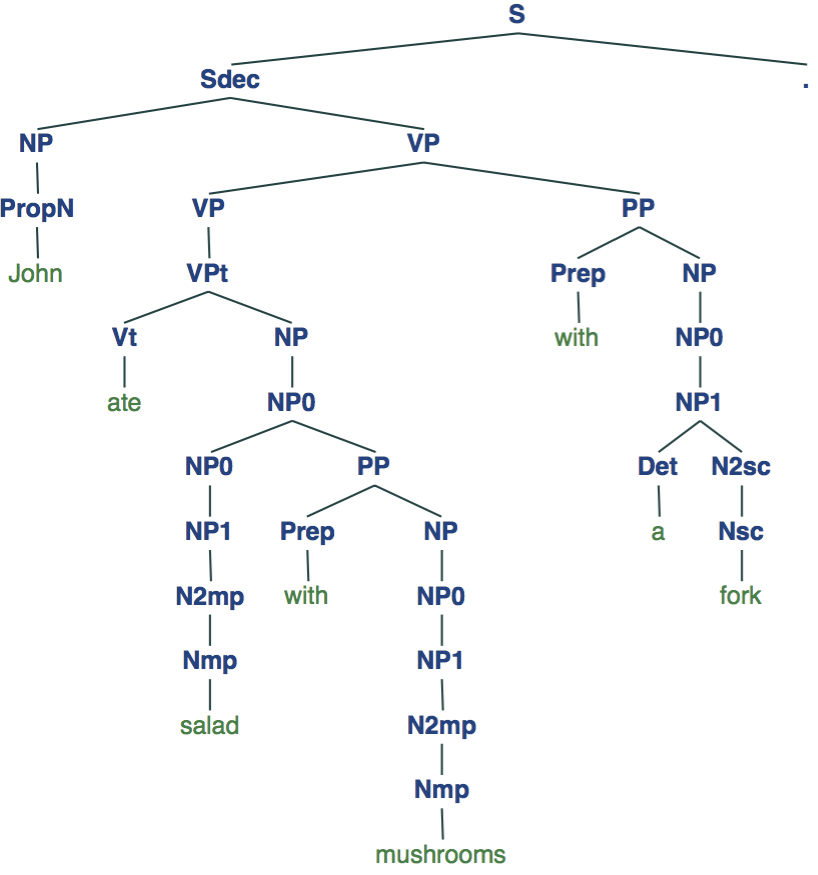
\includegraphics[width=0.4\linewidth]{../s4}
	\caption{\emph{John ate salad with mushrooms with a fork.}}
	\label{fig:s4}
\end{figure}
\begin{figure}[h!]
	\centering
	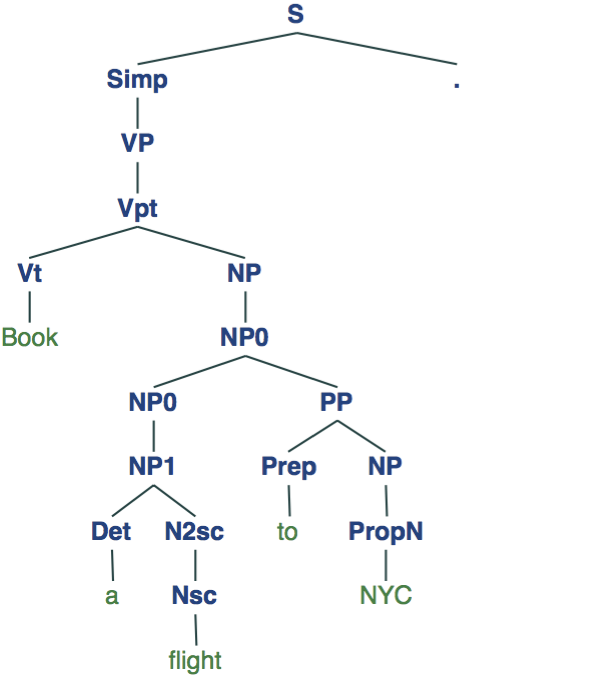
\includegraphics[width=0.4\linewidth]{../s5}
	\caption{\emph{Book a flight to NYC.}}
	\label{fig:s5}
\end{figure}
\begin{figure}[h!]
	\centering
	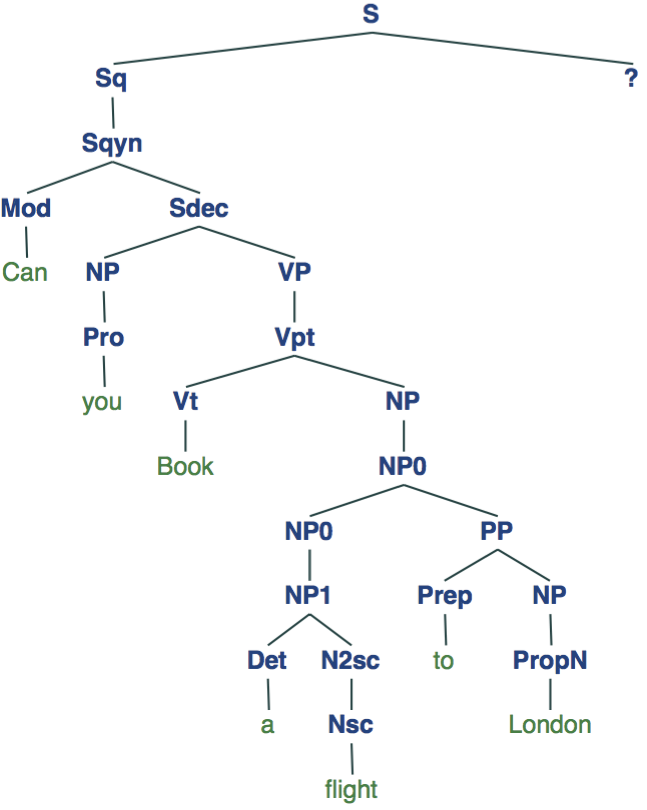
\includegraphics[width=0.4\linewidth]{../s6}
	\caption{\emph{Can you book a flight to London?}}
	\label{fig:s6}
\end{figure}
\begin{figure}[h!]
	\centering
	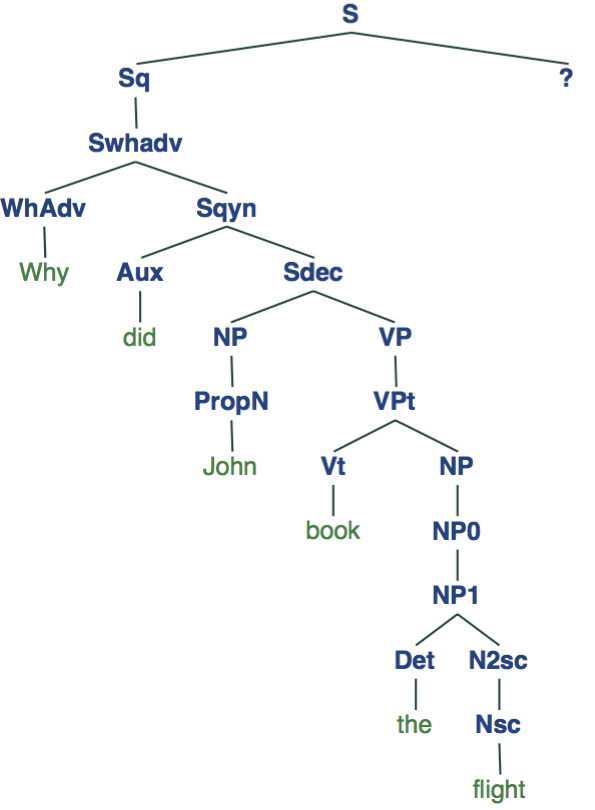
\includegraphics[width=0.4\linewidth]{../s7}
	\caption{\emph{Why did John book a the flight?}}
	\label{fig:s7}
\end{figure}
\begin{figure}[h!]
	\centering
	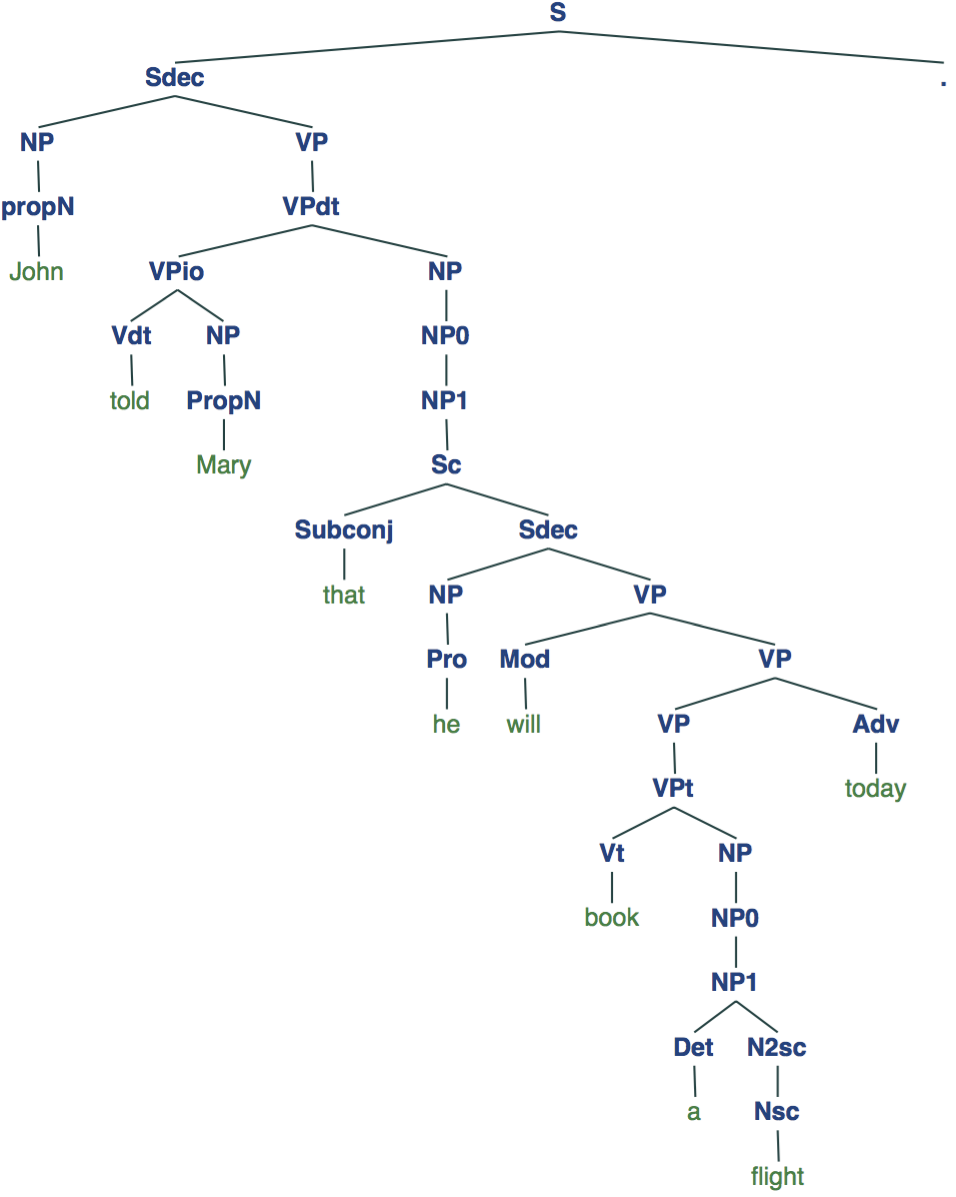
\includegraphics[width=0.4\linewidth]{../s8}
	\caption{\emph{John told Mary that he will book a flight today.}}
	\label{fig:s8}
\end{figure}

%----------------------------------------------------------------------------------------
%	QUESTION 3
%----------------------------------------------------------------------------------------
\section{Remarks on the grammar}

\begin{description}
	\item[Design of the grammar rules]
	\item[Positive aspects]
	\item[Negative aspects]
	
	\begin{enumerate}
		\item
		\textbf{Redundancy of rules in the verbal domain}
		
		There is a redundancy in the treatment of ditransitive verb phrases. \emph{VPo} an \emph{VPio} are two nodes which expand in the exact same way:
		\begin{center}
			
			\emph{VPo $\rightarrow$ Vdt NP} and \emph{VPio $\rightarrow$ Vdt NP}.
			
		\end{center}
		and therefore there is no difference between them within the grammar. From a linguistic point of view this separation might have a motivation. The ditransitive verb and its direct object are represented by \emph{Po}, while \emph{VPio} is a unit consisting of a ditransitive verb and its indirect object. As valid linguistic distinction as it might be, it does not need to be included in simple grammar like the one discussed here. In particular, no use is made of the distinction between that would limit overgenration. If that was the case, then having both non-terminals would be a valid design choice. For instance, one might consider putting some restrictions on what kinds of NP can be direct or indirect objects.
		The needless distinction between \emph{VPo} an \emph{VPio} propagates up to the topmost VP expansion rules. As a result, there are more VP-related rules than necessary. The grammar contains
		\begin{center}
			
			\emph{VP $\rightarrow$ VPi $\vert$ VPt $\vert$ VPdt $\vert$ Mod VP $\vert$ VP Adv $\vert$ VP PP}
			
			\emph{VPdt $\rightarrow$ VPo PP}
			
			\emph{VPdt $\rightarrow$ VPio NP}
			
			\emph{VPo $\rightarrow$ Vdt NP}
			
			\emph{VPio $\rightarrow$ Vdt NP}
			
		\end{center}
		but it could have contained as little as three rules instead:
		
		\begin{center}
			
			\emph{VP $\rightarrow$ VPi $\vert$ VPt $\vert$ VPdt $\vert$ Mod VP $\vert$ VP Adv $\vert$ VP PP}
			
			\emph{VPdt $\rightarrow$ VPd NP $\vert$ VPd PP}
			
			\emph{VPd $\rightarrow$ Vdt NP}
			
		\end{center}
		
		\item
		\textbf{Redundancy of rules in the nominal domain}
		
		Similarly, the NP0 non-terminal node seems redundant. It's purpose is to allow for recursive generation of prepositional phrases following a noun phrase. This can be achieved by accounting for this kind of recursion within one of the existinf NP rules. We could propose:
		
		\begin{center}
			
			NP $\rightarrow$ PropN $\vert$ Pro $\vert$ NP1 $\vert$ NP PP
			
			NP1 $\rightarrow$ Det N2sc $\vert$ N2mp $\vert$ Sc $\vert$ NP1 PP
			
		\end{center}
		
		The first option has the advantage of allowing for proper names and pronouns to be modified by prepositional phrases, which could be desirable in a more comprehensive grammar, however is not necessary for the grammar at hand. The second proposition is more conservative in that it would not lead to generating any string the original grammar doesn't. The 
		\begin{center}
			
			\emph{NP0 $\rightarrow$ NP1 $\vert$ NP0 PP}
			
		\end{center}
		rule expands to an \emph{NP1} followed by an arbitrary number of \emph{PPs}. The same effect will be achieved by adding the \emph{NP1 -> NP1 PP} expansion, with the benefit of reducing the number of non-terminals.
		One might argue that the \emph{NP0} node corresponds approximately to an X' node in X-bar syntax, and hence is theoretically justified. This, however, would need to mean that PPs to the right of the head noun are adjuncts rather than complements of that noun, which is not true. [TODO citation]
		
		\item
		\textbf{Dobtfull usefulness of the \textit{Sq} node}
		
		The \emph{Sq} node serves no purpose other than to reflect the conceptual relation between \emph{Sqyn} and \emph{Swhadv}, namely the fact both are non-terminals expanding into questions. This, however, represents only a superficial, if not mistaken, grammatical insight. In fact wh-questions and auxiliary-inversion questions are represented by very different structures (WH-phrases and Aux-phrases respectively[TODO citation]). If the motivation for including the \emph{Sq} node it linguistic, then the reasons seem insufficient.
		If, one the other hand, the node was included in the grammar to simplify the expansion of \emph{S}, then by analogy we should also include
		\begin{center}
			
			\emph{Sd $\rightarrow$ Sdec $\vert$ Simp}
			
		\end{center}an change the expansion of \emph{S} to
		\begin{center}
			
			\emph{S $\rightarrow$ Sd '.' $\vert$ Sq '?'}
			
		\end{center}
		
		\item
		\textbf{Lower case and capitalized versions of terminals.}
		
		It does not seem necessary to include lower case and capitalized versions of the same terminals. In the sample sentences we have seen \textit{Book, Can}, and \textit{Why} being capitalized to account for their sentence-initial positions. instead of duplicating lexical items, we could simply capitalize  the first word of a generated sentence and ignore sentence-initial capitalization during parsing.
		There would be no ill effects of such a change, since every generated sentence is, by definition, grammatical. Every word which happens to be initial in a sentence produced by the grammar is allowed to be there. The additional confirmation of this fact in form of the word's capitalised version being present in the grammar is unnecessary.
	\end{enumerate}
	\item[Overgeneration]\newline
	\begin{enumerate}
		\item
		\textbf{Lack of subject-verb agreement}
		
		There’s distinction between single/count and plural/mass nouns, but no corresponding distinction in the verbal domain. The problem is somewhat masked by the fact that most of the included verbs are in past tense, where in English there are no subject-verb agreement phenomena. Nevertheless, we can see that the grammar would accept  \emph{*the fork book a flight.}, a sentence which ignores verb conjugation requirements.
		
		\item
		\textbf{Treating VP as full sentences}
		
		The rules:
		\begin{center}
			
			S $\rightarrow$ Simp ‘.’
			
			Simp $\rightarrow$ VP
			
		\end{center}
		imply that any \emph{VP} can be a grammatical sentence on its own. This, however, is true only of \emph{VP} in imperative mood. The grammar, however, allows for treating any \emph{VP}, e.g. \emph{*ate today}, as a full sentence. Solving this problem is not possible without substantially expanding the grammar. We would have to distinguish between infinitival and inflected forms of verbs, and extend the set of possible expansions of \emph{VP} accordingly. We could then state that \emph{Simp} subcategories for \emph{VPs} whose head is an infinitival form of a verb. Therefore, we would need the following rules:
		\begin{center}
			
			Vt_inf $\rightarrow$ ‘Book’ $\vert$ ‘Tell’ $\vert$ …
			
			VPi_inf $\rightarrow$ ‘Eat' $\vert$ …
			
			VPt_inf $\rightarrow$ Vt_inf NP $\vert$ VPt_inf Adv $\vert$ VPt_inf PP
			
			VP $\rightarrow$ VPt_inf
			
			Simp $\rightarrow$ VPt_inf $\vert$ VPi_inf
			
		\end{center}
		Even then, additional restrictions would be needed to account for characteristics of the imperative mood, e.g. the fact that the second person pronoun needs to be in its reflexive form when used as a direct object of the matrix verb [TODO citation] . Otherwise the grammar would generate sentences such as \emph{*Book you a flight to London.} instead of grammatical \emph{*Book yourself a flight to London.}
		
		\item
		\textbf{Case agreement}
		
		The grammar does not account for case subcategorisation requirements of verbs. The only corner of the modern English syntax which still exhibits case phenomena is the pronoun system[TODO citation], however the grammar does not include a \emph{ProNom} and a \emph{ProAcc} pre-terminals. Having no distinction between nominative and accusative forms leads to admitting non-grammatical sentences, e.g.\emph{*Mary gave \textbf{he} a nice salad.} instead of \emph{Mary gave \textbf{him} a nice salad.}
		
		\item
		\textbf{Verb and noun subcategorization for pronouns}
		
		Verbs an nouns tend to co-occur with particular pronouns more often than with others. However, the grammar does not account for this preference. For instance, one can \emph{eat with a fork}, \emph{eat with Mary}, or have a \emph{flight to London}, but the grammar also allows for having a \emph{*salad to fork} and booking a \emph{*flight with NYC.}
		
		\item
		\textbf{Multiple modals}
		
		The grammar allows for an unlimited number of modals to proceed a \emph{VP}. This can lead to generating sentences such as \emph{*Can will can can John book a flight?}. However, English limits the acceptable number (up to 4, depending on dialetct), orderings (evidential, epistemic, deontic), and identity (\emph{might} or \emph{may} being the most commonly first in the sequence (Di Paolo 1989)) of verbs in multiple modal constructions. In order to capture these restrictions we would need a whole series of serially connected expansion rules, each introducing one modal of a certain type.
	\end{enumerate}
\end{description}

%----------------------------------------------------------------------------------------
%	QUESTION 7
%----------------------------------------------------------------------------------------

\section{Ambiguity Analysis}

\subsection{"John gave a book to Mary."}

\begin{description}
	\item[Distinct Parse(s):]
	3
	\item[Ambiguity Source:]
	
\end{description}

\subsection{"John gave Mary a book."}

\begin{description}
	\item[Distinct Parse(s):]
	1
	\item[Ambiguity Source:]
	
\end{description} 

\subsection{"John gave Mary a nice drawing book."}

\begin{description}
	\item[Distinct Parse(s):]
	2
	\item[Ambiguity Source:]
	
\end{description} 

\subsection{"John ate salad with mushrooms with a fork."}

\begin{description}
	\item[Distinct Parse(s):]
	5
	\item[Ambiguity Source:]
	
\end{description}

\subsection{"Book a flight to NYC."}

\begin{description}
	\item[Distinct Parse(s):]
	2
	\item[Ambiguity Source:]
	
\end{description}

\subsection{"Can you book a flight to London?"}

\begin{description}
	\item[Distinct Parse(s):]
	2
	\item[Ambiguity Source:]
	
\end{description}

\subsection{"Why did John book the flight?"}

\begin{description}
	\item[Distinct Parse(s):]
	1
	\item[Ambiguity Source:]
	
\end{description}

\subsection{"John told Mary that he will book a flight today."}

\begin{description}
	\item[Distinct Parse(s):]
	3
	\item[Ambiguity Source:]
	
\end{description}

%----------------------------------------------------------------------------------------
%	BIBLIOGRAPHY
%----------------------------------------------------------------------------------------

\bibliographystyle{apalike}

\bibliography{sample}

%----------------------------------------------------------------------------------------


\end{document}